\documentclass{standalone}
\usepackage{tikz}

\begin{document}

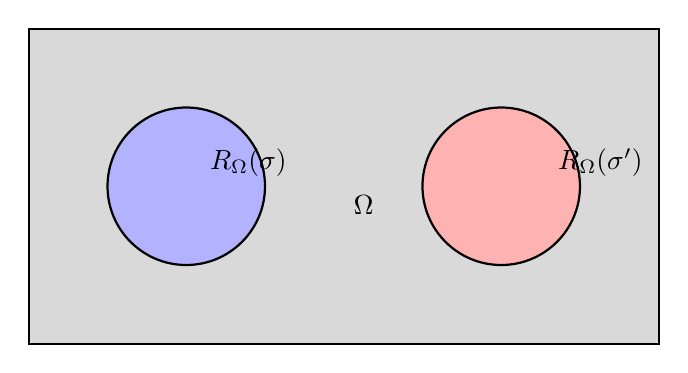
\begin{tikzpicture}[scale=2]
    % Draw the domain Ω as a rectangle
    \draw[thick, fill=gray!30] (0,0) rectangle (4,2);
    
    % Label the domain Ω
    \node at (2,1) [below right] {$\Omega$};
    
    % Draw the first circle for R_Ω(σ)
    \draw[thick, fill=blue!30] (1,1) circle (0.5);
    
    % Label the first circle
    \node at (1.7,1) [above left] {$R_\Omega(\sigma)$};
    
    % Draw the second circle for R_Ω(σ')
    \draw[thick, fill=red!30] (3,1) circle (0.5);
    
    % Label the second circle
    \node at (3.3,1) [above right] {$R_\Omega(\sigma')$};
\end{tikzpicture}

\end{document}